\pagebreak

\section{Modelo físico}
\subsection{Prueba de concepto}

Se construyó un péndulo simple empleando 
el paquete de construcción de LEGO Mindstorms.
Este paquete posee varias características
útiles para el estudio del sistema:
\begin{itemize}
 \item Unidad de computación integrada y programable.
 \item Modularidad de sus piezas.
 \item Facilidad de ensamble.
 \item Motores de corriente directa incluyen 
 codificadores rotatorios para retroalimentación.
\end{itemize}

\subsection{Análisis de video}

Se realizó un análisis de video del péndulo construido con 
el software de \emph{Tracker}\footnote{\url{https://www.physlets.org/tracker/}}.
El video fue grabado a 30 cuadros por segundo (fps) en resolución HD.
La figura \ref{fig: tracker theta} la posición angular del 
péndulo respecto al eje vertical, medido en radianes.
El diagrama de fase (figura \ref{fig: tracker phase diagram theta dtheta})
concuerda con el comportamiento observado en el diagrama de fase de 
la simulación con fricción.


\begin{figure}[htb!]
 \centering
%  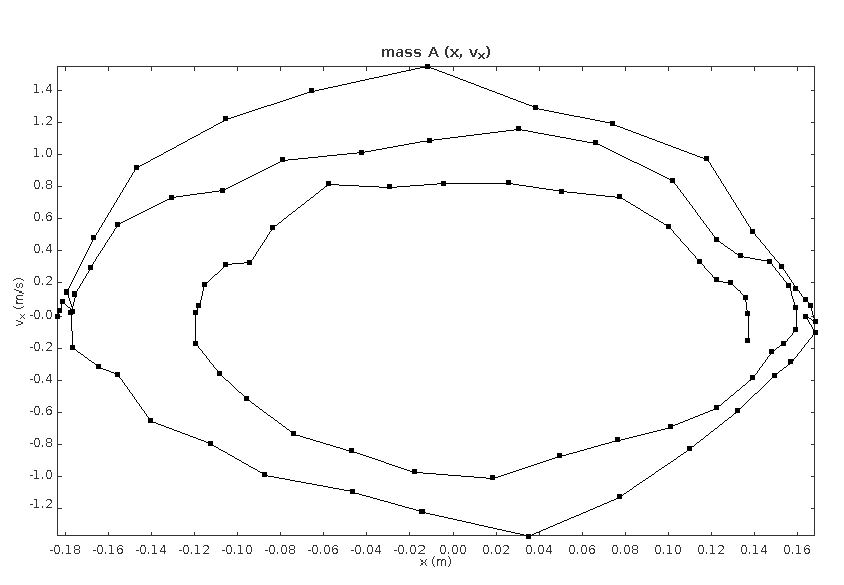
\includegraphics[scale=0.4]{./img/tracker_poc_phasediagram_x_vx.png}
\import{./img/}{pendulum_theta_tracker.pdf_tex}
 % tracker_poc_phasediagram_x_vx.png: 844x585 px, 72dpi, 29.78x20.64 cm, bb=0 0 844 585
 \caption{Diagrama de fase del modelo físico para $x$ y $\dot{x}$}
 \label{fig: tracker theta}
\end{figure}

\begin{figure}[htb!]
 \centering
%  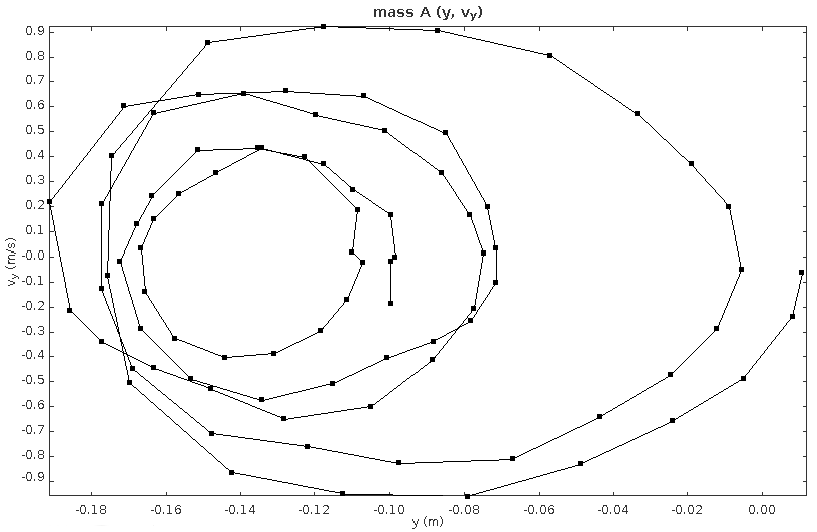
\includegraphics[scale=0.4]{./img/tracker_poc_phasediagram_y_vy.png}
\import{./img/}{pendulum_phase_tracker.pdf_tex}
 % tracker_poc_phasediagram_x_vx.png: 844x585 px, 72dpi, 29.78x20.64 cm, bb=0 0 844 585
 \caption{Diagrama de fase del modelo físico para $\theta$ y $\dot \theta$}
 \label{fig: tracker phase diagram theta dtheta}
\end{figure}


\subsection{Mediciones físicas}

Empleando los sensores incluidos en el paquete de LEGO
Mindstorms, fue posible realizar mediciones de la 
posición angular del péndulo para comparar con el
modelo matemático y el análisis de video.
La figura \ref{fig: mindstorms theta} muestra la
gráfica de mediciones de $\theta$ respecto al tiempo.
Se observa que las mediciones realizadas por el sensor
fueron afectadas por el nivel de ruido introducido 
por el mismo sensor.

\begin{figure}[htb!]
 \centering
%  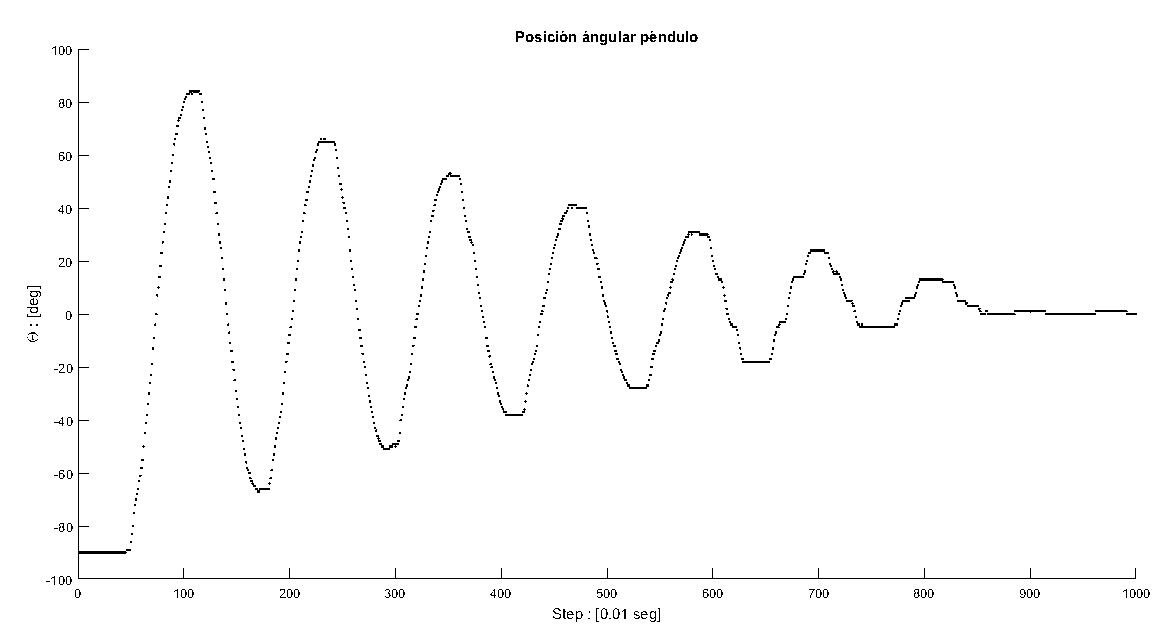
\includegraphics[scale=0.4]{../Mindstorms/Pendulin2_bw.png}
\import{./img/}{lego.tex}
 % Pendulin2_bw.png: 1157x625 px, 96dpi, 30.61x16.53 cm, bb=0 0 868 469
 \caption{Mediciones de $\theta$ para el péndulo físico con el codificador rotatorio.}
 \label{fig: mindstorms theta}
\end{figure}


\clearpage
